\textbf{Overview.} Similar to prior long-term planning work in open-world environments \citep{AhnBBCC2022, WangCMLJLM2024}, our approach, SCOPE, adopts a hierarchical agent design consisting of an employee agent for low-level execution and a manager agent for high-level planning. The manager agent proposes a high-level plan based on the current environment state and the ultimate goal, and then delegates control to the employee agent. The employee agent interacts directly with the environment to complete the assigned subgoals and returns control to the manager either upon completion or once a preset step limit is reached. This iterative process continues as the manager proposes subsequent subgoals, and terminates once the ultimate goal has been achieved. 

The remainder of this section describes how both agents are trained. Each agent is first pretrained on the suboptimal trajectories, followed by a reinforcement learning-based stage to further improve the goal-achievement rate. The RL training relies on interactions with world models. For the employee agent, the elementary world model is obtained by training directly on the provided suboptimal trajectories. The world model used for training the manager agent is then constructed by combining the trained employee agent with the elementary world model; its implementation details will be presented in the manager training section.


\subsection{Employee Agent}
The employee agent is responsible for accomplishing individual subgoals and is trained in two stages: an imitation-based pretraining phase to mimic suboptimal trajectories, followed by RL fine-tuning to maximize subgoal completion rate.

\textbf{Pretraining.} For pretraining, the agent $\pi^e_{\thetav}$  is trained to imitate suboptimal trajectories collected from human players by minimizing 
\begin{align}
	J^e(\thetav) = - \sum_{(s, a, \tilde g, I) \in \Phi} \log \pi^e_{\thetav}(a \vert s, \tilde g, I). 
\end{align}
This objective encourages the policy \(\pi^e_{\thetav}\) to reproduce the demonstrated behaviour, allowing it to learn an initial mapping from states and subgoals to actions under the given instruction.

\begin{figure*}
    \centering
    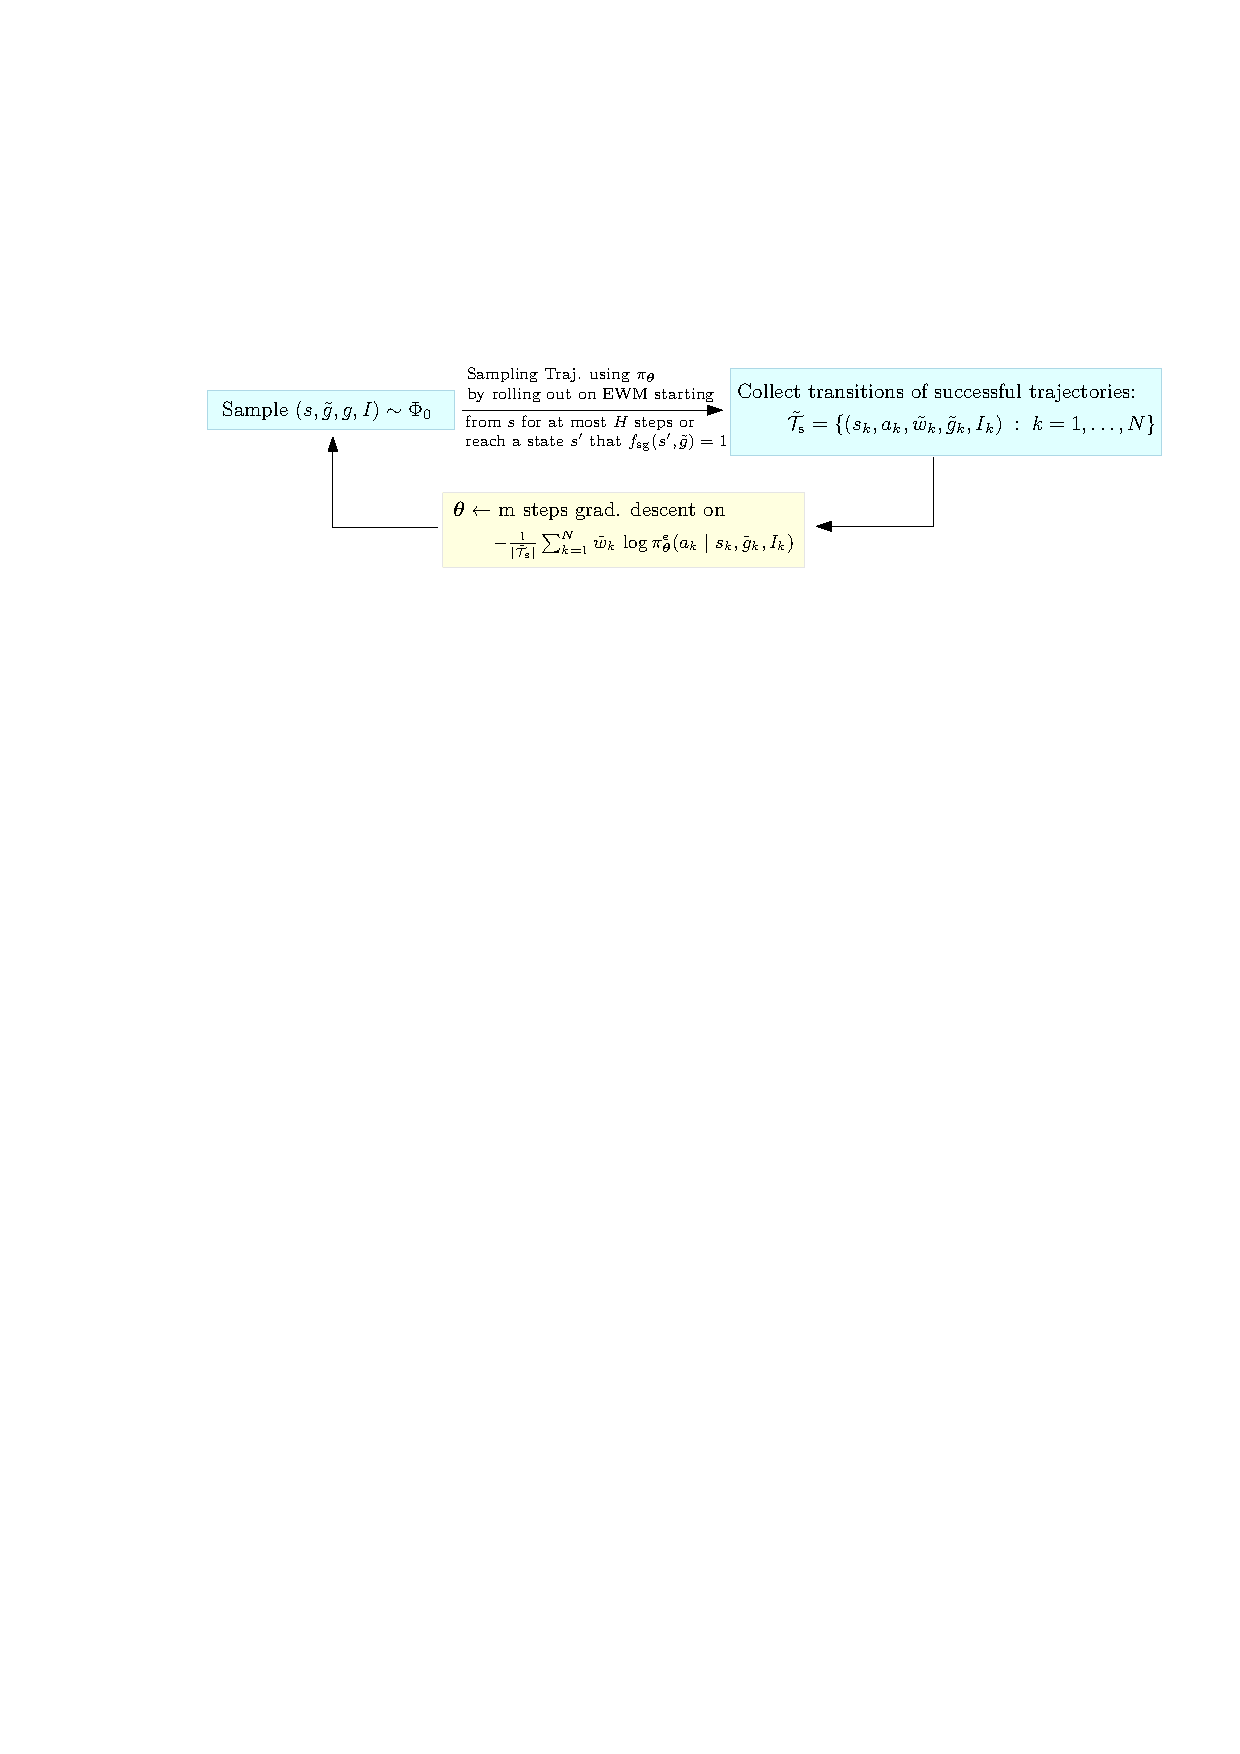
\includegraphics[width=0.9\textwidth]{figs/hier_agent_diagram.pdf}
    \caption{The RL training pipeline of the employee agent.}
    \label{fig:method}
\end{figure*}%
\textbf{Employee World Model.} The RL training builds on a world model trained from suboptimal trajectories to predict the next state and check action validity. Given the current state \(s\), action \(a\), and instruction \(I\), the elementary world model \(\EWM(s, a; I)\) first verifies whether \(a\) is valid. In TextCraft, an action is invalid if it cannot be parsed (e.g., semantically incorrect) or executed, for example, when a crafting command is missing from \(I\) or when the inventory lacks the required materials. If valid, the model predicts the next state; otherwise, it returns the current state, treating the action as rejected. It outputs both the next state and the validity flag. Since the state in TextCraft is represented as an inventory dictionary, we employ a neural network that takes \((s, a; I)\) in text form to predict only the action validity, while the next-state update is implemented directly through set operations. 


\textbf{RL Finetuning.} In this stage, the employee agent is further trained to maximize the expected subgoal achievement rate by interacting with the world model  \(\EWM(s, a; I)\). We use $f_{sg}$ function provided by the LLM-planner to check if a subgoal is completed. In our implementation, we adopt the Cross-Entropy Method (CEM,  \citealt{MannorRG2003,deBoerKMR2005}), a widely used derivative-free model-based RL (MBRL) algorithm that has demonstrated strong performance across challenging benchmarks \citep{WangB2020,YangCIZTS2020}. As illustrated in \cref{fig:method}, at each iteration the employee agent samples a random tuple $(s, \tilde{g}, g, I) \in \Phi_0$ and performs a rollout in the world model starting from $s$, which results in a new trajectory by executing a sequence of actions sampled from its policy network, conditioned on the current state, subgoal $\tilde{g}$ and instruction $I$. A total of $\Nc_e$ trajectories are sampled per iteration.


If a trajectory reaches a state \(s'\) such that \(f_{\mathrm{sg}}(s',\tilde g)=1\) within a preset number of steps, then each state-action pair \((s,a)\) in that trajectory is assigned the normalized weight
\(
\tilde w = \frac{1}{\lvert \text{traj} \rvert},
\)
where \(\lvert \text{traj} \rvert\) denotes the number of transitions; otherwise, the weight is set to zero. This scheme penalizes unnecessarily long trajectories and encourages achieving the subgoal with fewer steps. Collecting all weighted state-action pairs from successful trajectories yields
\[
\tilde \Tc_{\mathrm{s}}
= \big\{ (s_k, a_k, \tilde w_k, \tilde g_k, I_k) \;:\; k=1,2, \ldots,  \big\}
\]
where each tuple contains a state-action pair together with its assigned weight \(\tilde w_k\), the associated subgoal \(\tilde g_k\), and instruction \(I_k\). If $\tilde \Tc_\mathrm{s}$ is non-empty, the policy parameters $\thetav$ are then updated by minimizing the weighted negative log-likelihood over $\tilde  \Tc_{\mathrm{s}}$:
\begin{equation}
-  \frac{1}{|\tilde  \Tc_{\mathrm{s}}|}\sum_k
\tilde w_{k} \, \log \pi^e_{\thetav}(a_k \mid s_k, \tilde g_k, I_k),
\end{equation}
for a preset number of gradient descent steps, where $|\tilde  \Tc_{\mathrm{s}}|$ denotes the total number of tuples in $\tilde \Tc_{\mathrm{s}}$; otherwise, the update is skipped.  The process is repeated by resampling a new set of $\Nc_e$ trajectories. 


\subsection{Manager Agent}
Unlike the employee agent, which selects actions that directly interact with the environment, the manager agent proposes the next subgoal based on the current state and the ultimate goal, guiding the employee toward achieving that final goal.

\textbf{Pretraining.} For pretraining, the manager agent is trained to autoregressively reproduce the subgoal sequences generated by $f_{\text{dc}}(I, T)$ for $(g, I, T) \in \mathcal{S}$. This can be achieved by minimizing
\begin{align}
    \mathcal{J}^m(\boldsymbol{\phi})
    = - \sum_{(g, I, T) \in \mathcal{S}} \; \sum_{k = 1}^{N_T}
        ~~\log \pi_{\boldsymbol{\phi}}^{m} \big( \tilde{g}_k \mid s_{i_{k-1}}, g, I \big).
\end{align}
In this way, the manager agent acquires an initial ability to propose subgoals for each subtrajectory, conditioned on its initial state \(s_{i_{k-1}}\), the ultimate goal \(g\), and the accompanying instruction \(I\). This pretrained policy serves as a reasonable starting point, but is not expected to be optimal. 

%In other words, the manager agent learns to propose the appropriate subgoal for each subtrajectory, conditioned on its initial state $s_{i_{k-1}}$, the ultimate goal $g$, and the accompanying instruction $I$.

%After pretraining, the manager agent is then further optimized using RL methods to maximize the ultimate goal-achievement rate. This stage relies on rolling out trajectories within a world model operating at the subgoal level. We show that this manager-level world model can be constructed by combining the employee world model \(\EWM\) with the trained employee agent \(\pi^{e}_{\thetav}\) that the manager needs to collaborate with. 

After pretraining, the manager agent is further optimized using RL to maximize the ultimate goal-achievement rate. This stage involves rolling out trajectories within a world model that operates at the subgoal level. We show that this manager-level world model can be constructed by combining the employee world model \(\EWM\) with the trained employee agent \(\pi^{e}_{\thetav}\), which the manager needs to coordinate with during planning.

\textbf{Manager World Model.} In contrast to the employee world model, the manager world model treats subgoals as actions. Therefore, correspondingly, the manager world model $\MWM(s, \tilde{g})$ takes the current state $s$ and a proposed subgoal $\tilde{g}$ as input and first checks whether $\tilde{g}$ is achievable within a preset number of steps. If so, it returns the resulting state upon subgoal completion; otherwise, it returns $s$. Here, ``achievable'' means that the subgoal is both plausible and executable by the deployed employee agent. To implement this, we roll out the employee policy \(\pi_{\thetav}^e\) on the employee world model \(\EWM\) starting from \(s\). If \(\tilde{g}\) is reached within the step limit, the final state is returned; otherwise, the initial state is returned.

To determine whether the ultimate goal is achieved, we can use an ultimate-goal completion function $f_{\text{ug}}(s, g)$, which returns $1$ if the ultimate goal $g$ is satisfied in state $s$ and $0$ otherwise. In general, $f_{\text{ug}}$ can be implemented using a neural network trained via supervised learning on the provided suboptimal trajectories. In TextCraft, however, it can be computed directly by checking whether the inventory contains the ace item.


\textbf{RL Finetuning.} 
In the RL stage, the manager agent is trained in a manner similar to the employee agent, but operates at the subgoal-proposing level by interacting with $\MWM$. In particular, at each iteration, the manager agent samples a random tuple $(s,\tilde g, g, I) \in \Phi_0$ and performs a rollout in $\MWM$ starting from $s$.\footnote{During RL fine-tuning, subgoals are drawn from $\pi^m_{\phiv}(\cdot \mid s, g, I)$, and the $\tilde g$ in $\Phi_0$ is not used.} The rollout ends when either a preset maximum number of steps is reached or the ultimate goal $g$ is achieved. This produces a new state-subgoal trajectory $(s_0, \tilde g_0, s_1, \tilde g_1, \ldots, s_{l-1}, \tilde g_{l-1}, s_l)$, where $s_0 = s$ and $l$ is the total number of proposed subgoals. If $f_{\mathrm{ug}}(s_l, g) = 1$, the trajectory is considered successful and each state-subgoal pair $(s_k, a_k)$ for $k = 0,1,\ldots,l-1$ is assigned a normalized weight $w = \frac{1}{l}$. Otherwise, the trajectory is treated as a failure, and all state-subgoal pairs receive weight zero.  Similar to the RL finetuning of the employee agent, this scheme penalizes unnecessarily long trajectories and encourages achieving the ultimate goal with a smaller number of subgoals. At each iteration, $\Nc_m$ trajectories are generated. Gathering the weighted state-subgoal pairs from all successful trajectories yields
\[
\Tc_{\mathrm{s}}
= \big\{ (s_k, \tilde{g}_k, w_k, g_k, I_k) \;:\; k=1,2, \ldots  \big\},
\]
where each tuple contains a state-subgoal pair together with its assigned weight \(w_k\), the associated ultimate goal \(g_k\), and instruction \(I_k\). If $\Tc_\mathrm{s}$ is non-empty, the policy parameters $\phiv$ are then updated by minimizing the weighted negative log-likelihood over $\Tc_{\mathrm{s}}$:
\begin{equation}
-  \frac{1}{|\Tc_{\mathrm{s}}|}\sum_k
w_{k} \, \log \pi^m_{\phiv}(\tilde g_k \mid s_k, g_k, I_k),
\end{equation}
for a specified number of gradient updates, with $|\Tc_{\mathrm{s}}|$ indicating the number of tuples in the set. If $\Tc_{\mathrm{s}}$ is empty, no update is performed. The procedure then continues by sampling a fresh batch of $\Nc_m$ trajectories for the next iteration.


Upon completion of training, the manager and employee agents are combined in a hierarchical manner, as described earlier in this section, and deployed for evaluation in the environment. The effectiveness of this approach is demonstrated in \cref{sec:emp}.